\chapter{Results}\label{chp:chapter4}
\section{Survey responses}
As discussed previously, a participation rate of 35-48\% was necessary for a 10\% sampling error and 80\% confidence level. This allowed for inferences to be made on the population, not just the students sampled. The CS and IS senior classes were estimated by their respective departments to be one hundred students each, so participation from twenty-one students was necessary for each major. The IT senior class was estimated at forty students, requiring participation from sixteen students. Table~\ref{tab:response-rates} shows the amount of responses received compared to the total amounts needed.

\begin{table}[h!]
  \centering
  \caption{Response Rates of Various Majors}
  \label{tab:response-rates}
  \begin{tabular}{llllll}
    \toprule
    Major & Total seniors in major & Surveys needed & Surveys received & Response rate\\
    \midrule
    CS    & 100                    & 35             & 40               & 40\%\\
    IS    & 100                    & 35             & 2                & 2\%\\
    IT    & 40                     & 14             & 22               & 55\%\\
    \bottomrule
  \end{tabular}
\end{table}

There were many complications getting responses from IS students. IS seniors do not have a capstone or senior seminar class, so there was no common opportunity to reach them. Since the Learning Style Inventory (LSI) is copyrighted and licensed for hardcopy use, it couldn't be digitized for distribution. This made it difficult to get surveys into the hands of the IS students. After trying for a year to get surveys out and being stonewalled by significant distribution problems, only two surveys from IS students were completed, and those were only completed because those students were in an IT course in which the surveys were distributed. No additional surveys were returned from IS students.

Because of the complications surrounding the IS responses, the IS results were not included in the analysis.

\section{What the LSI responses mean}
A student's strength on the two axes of the LSI can be seen in Figure~\ref{fig:learning-preferences} which defines the cognitive strengths throughout the LSI spectrum. These strengths can be either in abstract conceptualization (AC), active experimentation (AE), concrete experience (CE), reflective observation (RO), or along the AC-CE or AE-RO spectrums.

\begin{figure}
  \centering
  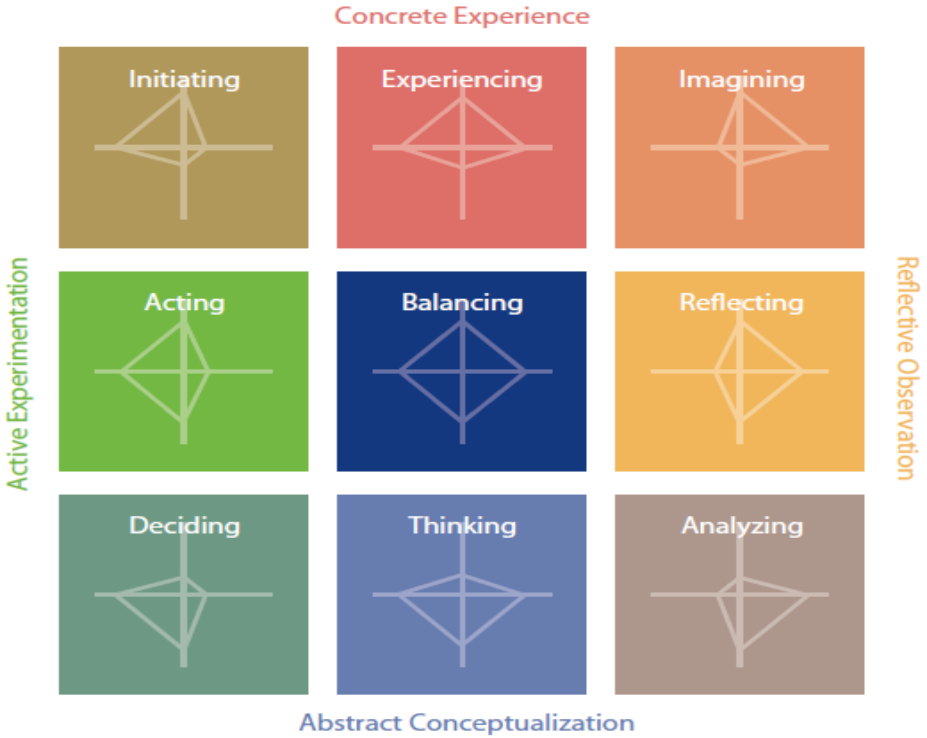
\includegraphics[width=0.9\textwidth]{figures/chapter4/learning-preferences.png}
  \caption{LSI Learning Preferences}
  \label{fig:learning-preferences}
\end{figure}

\subsection{Defining AC, CE, AE, and RO}
The terms abstract conceptualization, active experimentation, concrete experience, and reflective observation are not really intuitive. Before diving into the statistical analysis, it will be helpful to more clearly define these terms. The following list contains statements to help define each of these terms~(Kolb, 1993):
\begin{enumerate}
  \item Abstract conceptualization
  \begin{enumerate}
    \item To learn, I'd rather think about ideas.
    \item I'm logical.
    \item I like to reason things out.
    \item I want to analyze things.
    \item I'm rational.
    \item I rely on my ideas.
  \end{enumerate}
  \item Concrete experience
  \begin{enumerate}
    \item Thinking about my feelings affects how I learn.
    \item I trust my feelings and intuition.
    \item I'm open to experiencing new things.
    \item I like to learn from personal relationships.
    \item I like being actively involved in the learning process.
  \end{enumerate}
  \item Active experimentation
  \begin{enumerate}
    \item I want to be doing.
    \item I like to work hard.
    \item I want to see results.
    \item Just let me try it out myself.
    \item I'm practical.
  \end{enumerate}
  \item Reflective observation
  \begin{enumerate}
    \item I prefer to watch and listen.
    \item When I learn, I'm quiet.
    \item I take my time when I learn.
    \item I'm reserved.
    \item I like to look at issues from different angles.
    \item I'm observant.
    \item I prefer to slow down and be careful.
  \end{enumerate}
\end{enumerate}

\section{Answering the research questions}
\subsection{How strong is the correlation between AC-CE and AE-RO, and major GPA among CS, IS, and IT students?}
The first basic test was to calculate the Pearson correlation coefficient between AC-CE and AE-RO by major in order to check for a general correlation between learning preferences. The data failed to show a meaningful relationship between the two (the coefficient is $0.05496$, which with a \textit{p}-value of $0.733$ is not statistically significant). This is interesting because it goes against what the literature previously discussed about the relationship between learning styles, \textit{viz}.: CS and IT should be distinguishable~(Kolb, 2005b).

The next step was to check the simple correlation between AE-RO and AC-CE by major GPA. The Pearson coefficients are $0.4228$ ($p=0.0073$) and $-0.0101$ ($p=0.953$), respectively. This appears to show that the only significant relationship occurs in the AE-RO spectrum. Having high significance in the first Pearson coefficient says that there's a strong, positive relationship such that major GPA increases for students with higher AE-RO scores. However, there is no relationship between AC-CE score (the second Pearson coefficient) and major GPA. This means that students who have higher AE-RO scores will tend to perform better in either major; however, the AC-CE spectrum does not hold any statistically significant ($p>0.05$) effect on student GPA in CS or IT. This is interesting because Lunt found that AC-CE was the significant axis among electronics students~(Lunt, 1996).

\subsection{What is the best multiple regression model to fit these correlations?}
In order to estimate the relationship that AC-CE and AE-RO each have simultaneously, I developed a few multiple regression models. The first two models can be seen in Table~\ref{tab:models12} and are explained below.

\begin{table}[!htbp]
  \centering
  \caption{Models~1 and 2}
  \label{tab:models12}
  \begin{tabular}{@{\extracolsep{5pt}}lll}
  \toprule
   & \multicolumn{2}{c}{\textit{Dependent variable: Major GPA}} \\
  \cmidrule{2-3}
  \\[-1.8ex] & (1) & (2)\\
  \midrule
  CS dummy variable & 0.238$^{**}$ & 0.137 \\
    & (0.112) & (0.107) \\
    & & \\
  AC-CE & $-$0.001 & 0.0002 \\
    & (0.004) & (0.004) \\
    & & \\
  AE-RO & 0.007 & 0.007 \\
    & (0.006) & (0.005) \\
    & & \\
  \midrule
  Observations & 62 & 62 \\
  R$^{2}$ & 0.088 & 0.389 \\
  Adjusted R$^{2}$ & 0.040 & 0.269 \\
  Residual Std. Error & 0.418 (df = 58) & 0.365 (df = 51) \\
  F Statistic & 1.857 (df = 3; 58) & 3.250$^{***}$ (df = 10; 51) \\
  \bottomrule
  \textit{Note:}  & \multicolumn{2}{r}{$^{*}p<0.1$; $^{**}p<0.05$; $^{***}p<0.01$} \\
  \end{tabular}
\end{table}

For Model~1, I included the students' AC-CE and AE-RO scores, as well as a dummy variable that captured whether a student was a CS major. This model showed a significant correlation between AE-RO and GPA held even when controlling for the AC-CE value and the student's major with a very significant F statistic of $5.075$ (df$=3$, $p<0.01$). This F statistic showed that these factors were especially important in predicting a student's academic success, as measured by major GPA.

In Model~2, I used the same multiple regression analysis as Model~1, but added the student's age and their parents' education level as covariates. This correlation held, even when controlling for other factors that may have a relationship with GPA. This model had a strong F statistic, which again showed that the same factors, except for AC-CE, were significant in predicting a student's academic success.

In both models, however, AC-CE had a \textit{p}-value greater than $0.05$ which helped suggest that AC-CE was not a significant contributor to a student's academic success. Because the AC-CE values do not have a significant correlation with major GPA ($p>0.05$), they were dropped in the subsequent models.

In the next two models (see Table~\ref{tab:models34}), AE-RO was decomposed into its two individual elements because it was not clear which element was driving the AE-RO correlation with GPA. Model~3, which has AE-RO decomposed, showed that RO had a negative relationship with major GPA. When control variables (age and parents' education level) were added in Model~4, only the RO relationship remained statistically significant. These models are probably the best fit to estimate these correlations, with R-squared values of $0.304$ and $0.567$, respectively. The RO value and control terms have a high joint significance ($F=10.8$, $p<0.01$), so they should not be removed from the model. Model~4 had an adjusted R-squared of $0.4118$, meaning that the variables in the model can explain roughly 41\% of the variance in major GPA in this sample.

\begin{table}[!htbp] \centering
  \centering
  \caption{Models~3 and~4}
  \label{tab:models34}
  \begin{tabular}{@{\extracolsep{5pt}}lll}
    \toprule
     & \multicolumn{2}{c}{\textit{Dependent variable: Major GPA}} \\
    \cmidrule{2-3}
    \\[-1.8ex] & (1) & (2)\\
    \midrule
    csdum & 0.231$^{**}$ & 0.135 \\
      & (0.109) & (0.103) \\
      & & \\
    RO.total & $-$0.018$^{**}$ & $-$0.021$^{**}$ \\
      & (0.009) & (0.009) \\
      & & \\
    AE.total & $-$0.003 & $-$0.004 \\
      & (0.008) & (0.008) \\
      & & \\
    \midrule
    Observations & 62 & 62 \\
    R$^{2}$ & 0.128 & 0.434 \\
    Adjusted R$^{2}$ & 0.083 & 0.323 \\
    Residual Std. Error & 0.409 (df = 58) & 0.351 (df = 51) \\
    F Statistic & 2.844$^{**}$ (df = 3; 58) & 3.912$^{***}$ (df = 10; 51) \\
    \bottomrule
    \textit{Note:}  & \multicolumn{2}{r}{$^{*}p<0.1$; $^{**}p<0.05$; $^{***}p<0.01$} \\
  \end{tabular}
\end{table}

The research question being examined here is: ``What is the best multiple regression model to fit these correlations?'' Models~3 and~4, with their high R-squared and F statistics, clearly show the best multiple regression models to find and fit these correlations. Model~4, with its adjusted R-squared, can explain over 41\% of the variance found in the models which helps show that the RO value is, statistically, the most important distinguisher between students' academic success in CS and IT.

Initial data analysis showed a significant correlation between RO and GPA, but I wanted to dig a bit deeper because it had the potential to show more information about whether the RO effect differed across majors. The following analysis is exploratory. Future research should be more explicit in the data analysis methods that will be used before this stage of the research.

Regressions were then run to check for the RO effect by major (summarized in Table~\ref{tab:models567}). The first step was to include an interaction term (Model~5) between the RO value and the CS dummy variable. This model captured whether the relationship between RO and major GPA was different between CS majors and IT majors. This term was statistically significant ($p<0.05$) with a negative relationship between RO and major GPA; however, it was unclear in which major that relationship occurs.

\begin{table}[!htbp]
  \centering
  \caption{Models~5, 6, and 7}
  \label{tab:models567}
  \begin{tabular}{@{\extracolsep{5pt}}llll}
    \toprule
     & \multicolumn{3}{c}{\textit{Dependent variable: Major GPA}} \\
    \cmidrule{2-4}
    \\[-1.8ex] & (1) & (2) & (3)\\
    \midrule
    csdum & $-$0.633 &  &  \\
      & (0.469) &  &  \\
      & & & \\
    RO.total & $-$0.038$^{***}$ & $-$0.005 & $-$0.043$^{***}$ \\
      & (0.013) & (0.011) & (0.013) \\
      & & & \\
    \midrule
    Observations & 62 & 40 & 22 \\
    R$^{2}$ & 0.461 & 0.005 & 0.341 \\
    Adjusted R$^{2}$ & 0.356 & $-$0.021 & 0.308 \\
    Residual Std. Error & 0.342 (df = 51) & 0.405 (df = 38) & 0.369 (df = 20) \\
    F Statistic & 4.369$^{***}$ (df = 10; 51) & 0.204 (df = 1; 38) & 10.337$^{***}$ (df = 1; 20) \\
    \bottomrule
    \textit{Note:}  & \multicolumn{3}{r}{$^{*}p<0.1$; $^{**}p<0.05$; $^{***}p<0.01$} \\
  \end{tabular}
\end{table}

In order to test this relationship by major, I ran two additional regression models (models~6 and~7) that focused on each major independently. In Model~5, I failed to find any statistical correlation between RO and major GPA among CS students, with the model on the whole failing joint significance, meaning that the variables are not statistically significant together.

In Model~7, focused solely on IT students, I found a significant, negative relationship between RO and major GPA. What this means is that moving from a low RO to a high RO (two standard deviations of RO scores) corresponds to a decrease of about $0.51$ in GPA. This is significant because it means that students who are more localized in RO will tend to have lower GPAs. Substantively, this is a lot. It's the difference between a $3.2$~GPA (the median IT GPA) and a $3.7$~GPA.

But what does that mean in the real world? Is that enough to make a difference in getting a job or getting into graduate school? There are certainly other factors contributing to that, but a $0.51$~GPA increase certainly has merit on its own. Looking deeper into it, the standard deviation of IT GPAs is $0.44$. The IT GPAs are pretty normally distributed, so this means that moving higher on the RO scale relates to more than an entire standard deviation decrease in GPA!

The fact that the RO low-to-high difference correlates to a little over one standard deviation means that the change is roughly comparable to decreasing roughly 38 percentiles from the mean (given that 68\% are within one standard deviation of the mean in either direction). This seems like it could be substantive, at least for IT students, since IT GPA is lower when the student more strongly prefers Reflective learning. However, this doesn't seem to hold for CS, as shown in Model~6.

\subsection{How strong is the correlation between AC-CE and AE-RO, and student satisfaction among CS, IS, and IT students?}
Nuata's AMSS, as enumerated in chapter 1, is graded on a five-point Likert-type scale with two of the responses being negatively scored. Two of the AMSS questions assume that students still have the option of changing their major, but once BYU students get beyond a certain credit threshold (well before their senior year), it becomes impossible for them to change majors. Because of this and the lack of variance among the responses, these questions were dropped from the analysis.

I created a summary index (Table~\ref{tab:nuata-summary-index}) of academic major satisfaction using the remaining AMSS variables and reverse coded the negatively-scored variables. In this summary index, the least satisfied value was a 4 and the most satisfied was a 20.

\begin{table}[!htb]
  \centering
  \caption{Summary Index of AMSS}
  \label{tab:nuata-summary-index}
  \begin{tabular}{cccccc}
    \toprule
    Min.  & 1st Qu. & Median & Mean  & 3rd Qu. &Max. \\
    \midrule
    12.00 &  16.25  & 19.00  & 18.10 & 20.00   & 20.00 \\
    \bottomrule
  \end{tabular}
\end{table}

Next, I checked the simple correlations between AE-RO and AC-CE with the satisfaction index. The Pearson coefficients are $-0.1206$ ($p=0.4645$) and $-0.0622$ ($p=0.7064$), respectively. It is possible that the relationship could only exist for the RO value, since this was the only value correlated with major GPA in the previous section. Checking for that, I found a Pearson correlation coefficient of $0.2634$ ($p=0.1051$). This means that even restricting to just RO and IT majors fails to find a statistically significant correlation ($0.2483$, $p=0.2652$).

None of these correlations were statistically significant, suggesting that there is no relationship between learning style and major satisfaction.

\subsection{Is there a correlation between major GPA and student satisfaction?}
The Pearson correlation coefficient of major GPA and the satisfaction index is $-0.1198$ ($p=0.4677$). This is statistically insignificant, so I am unable to say that there is a correlation between the two. The coefficient is negative, so if the correlation was significant it would indicate that students with higher major GPAs were generally less satisfied than students with lower GPAs.

% Add std dev
% Differentiate by major as well
The dataset, with four questions used, had a minimum sum of 4 (meaning the student strongly disagreed to each statement) and maximum sum of 20 (meaning the student strongly agreed with everything). The mean response was 18, so students were generally overwhelmingly satisfied with their choice of major. This lack of diversity is believed to have led to the lack of correlations between student satisfaction and other factors.

\section{Demographics}
Unfortunately, I was unable to use the full set of demographic variables collected from students as covariates because there was not enough variance among the sample group. The students were almost entirely white and male (88\% for both). Looking at the relationship between marital status and its relationship on major GPA and satisfaction had a multiple R-squared of $0.07$, and the relationship between marital status and RO and major GPA (previously the best model) had a multiple R-squared of $0.14$. So, while students were roughly equally divided in marital status, there was no relationship between marital status and any other factor.
